\documentclass{snedecorbeamer}

%% Figures
\usepackage{subcaption}

%% Captions
%%% Small font
\captionsetup{font=tiny}
%%% Remove caption
\setbeamertemplate{caption}{\raggedright\insertcaption\par}

%% Footnotes
%%% Small font https://tex.stackexchange.com/a/146021
\setbeamerfont{footnote}{size=\tiny}

% \setbeamertemplate{logo}{%
%     \usebeamercolor[fg]{footline}%
%     \usebeamerfont{page number in head/foot}%
%   \usebeamertemplate*{frame numbering}%
% }

%% Diagrams
%%% General tikz preamble
\usepackage{tikz}
\usetikzlibrary{positioning,decorations.pathreplacing,quotes,overlay-beamer-styles}

\newcommand{\citep}[1]{}

%% Create section slides
%%% https://tex.stackexchange.com/a/117661
\AtBeginSection{\frame{\sectionpage}}
\AtBeginSubsection{\frame{\subsectionpage}}

% Setup ------------------------------------------------------------------------
\graphicspath{{include/}}

\title{\textbf{Automatic Relevance Determination} \\
  for Gaussian Processes with Functional Inputs}

\renewcommand*{\thefootnote}{\fnsymbol{footnote}}
\author[Damiano et al]{
  \textbf{Luis Damiano}\footnote[2]{
    \tiny{\href{mailto:ldamiano@iastate.edu}{ldamiano@iastate.edu}}
  }}

\institute{
  Department of Statistics, Iowa State University
}

\date[December 19th, 2022]{
  \tiny{Argonne National Laboratory \\
    MCS Mathematics and Computer Science} \\
  December 19th, 2022}

\begin{document}

% Title page -------------------------------------------------------------------
\begin{frame}
  \titlepage{}
  {
    \tiny{
      Funded, in part, by
      \begin{itemize}
      \item[-] ISU Presidential Interdisciplinary
	Research Initiative on C-CHANGE:~Science for a Changing
	Agriculture
      \item[-] Foundation for Food and Agriculture Research
	Grant ID: CA18-SS-0000000278
      \end{itemize}
    }
  }
\end{frame}

% Introduction -----------------------------------------------------------------
%
\section{Motivation}

\begin{frame}
  \frametitle{Functional input computer models}
  \framesubtitle{A few examples}

  \begin{table}[]
    \footnotesize
    %\begin{tabular}{@{}lllll@{}}
    \begin{tabular}{p{15ex}p{20ex}p{15ex}p{20ex}p{15ex}}
%      \toprule
      \small Output
      & \begin{tabular}[c]{@{}l@{}}\small Input\\ $X(t): \mathcal{T} \to
	  \mathbb{R}$\end{tabular}
      & \begin{tabular}[c]{@{}l@{}}\small Index\\ $t \in \mathcal{T}$\end{tabular}
      & \begin{tabular}[c]{@{}l@{}}\small Index subspaces\\ $t \in
	  \mathcal{T}_u$\end{tabular}
      & \small Mechanism
      \\
      \midrule
      \only<1>{%
      Plant growth
      & Phosphorus
      & Depth
      & Soil layers
      & Root biomass \vspace{1ex}
      }
      \only<2>{%
      Soil erosion
      & Slope
      & Distance
      & Up/down hillslope
      & Water erosion \vspace{1ex}
      }
      \only<3>{%
      Radiance
      & Chemical species
      & Pressure
      & Atmospheric layers
      & Reflectivity \vspace{1ex}
      }
      \\
    \end{tabular}
  \end{table}

  \begin{figure}
    \centering
    \only<1>{%
      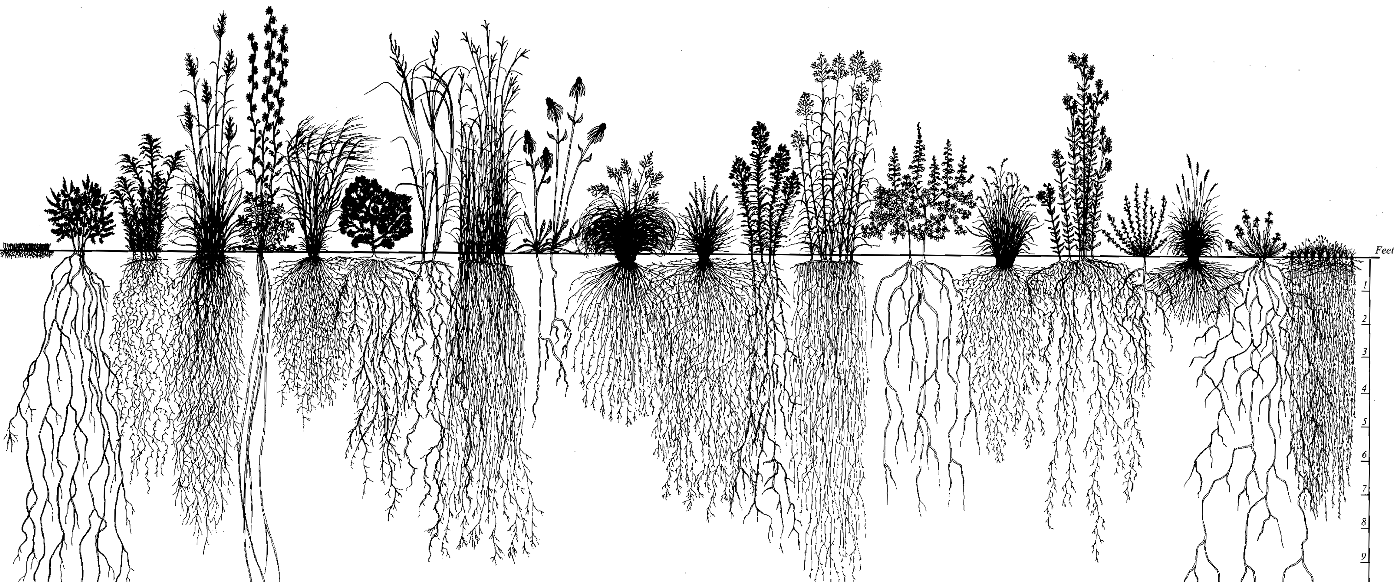
\includegraphics[height=12em]{inc/computer_model_roots_crop}
      \caption*{%
        \href{https://tallgrassprairiecenter.org/curriculum_images}{\resizebox{!}{1.5ex}{\beamergotobutton{www}}}
        Tallgrass Prairie Center}
    }
    \only<2>{%
      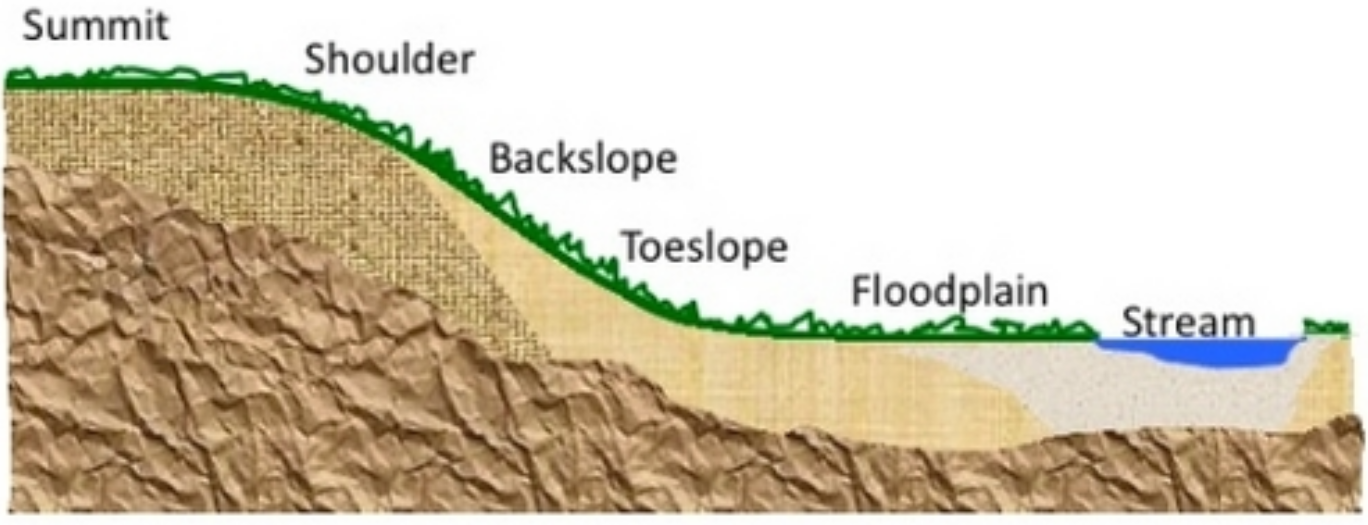
\includegraphics[height=12em]{inc/computer_model_hillslope_crop}
      \caption*{%
        \href{https://www.nature.com/scitable/knowledge/library/soil-carbon-storage-84223790/}{\resizebox{!}{1.5ex}{\beamergotobutton{www}}}
        Nature Education Knowledge (ask Brian Gelder)}
    }
    \only<3>{%
      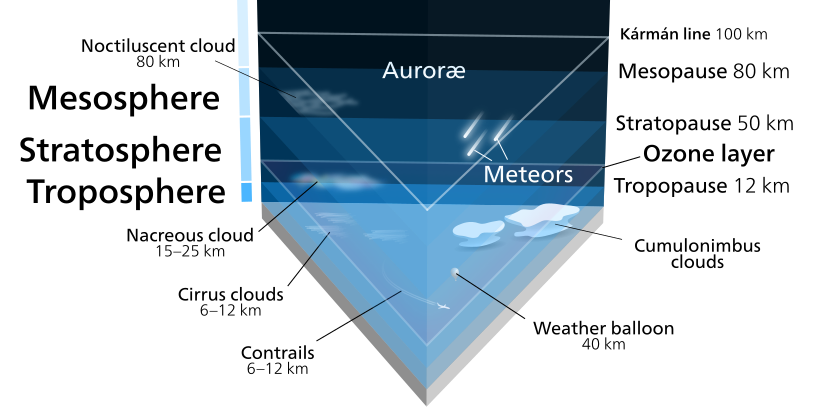
\includegraphics[height=12em]{inc/computer_model_atmosphere_crop}
      \caption*{%
        \href{https://commons.wikimedia.org/wiki/File:Earth's_atmosphere.svg}{\resizebox{!}{1.5ex}{\beamergotobutton{www}}}
        Wikimedia}
    }
  \end{figure}
\end{frame}

\begin{frame}
  \frametitle{Automatic Relevance Determination\cite{neal1998}}
  \framesubtitle{What is it?}

  $\mathrm{Cor}(y_i, y_j) = e^{\omega {(x_i - x_j)}^2}$
  where $\omega\in\mathbb{R}^+$ is a weight driving the response correlation

  \begin{itemize}
  \item A predictor has little contribution on prediction as $\omega\to0^+$
    (flat)
  \item A predictor contributes to local predictions as $\omega\to\infty$
    (wiggly)
  \end{itemize}

  \begin{figure}
    \centering
    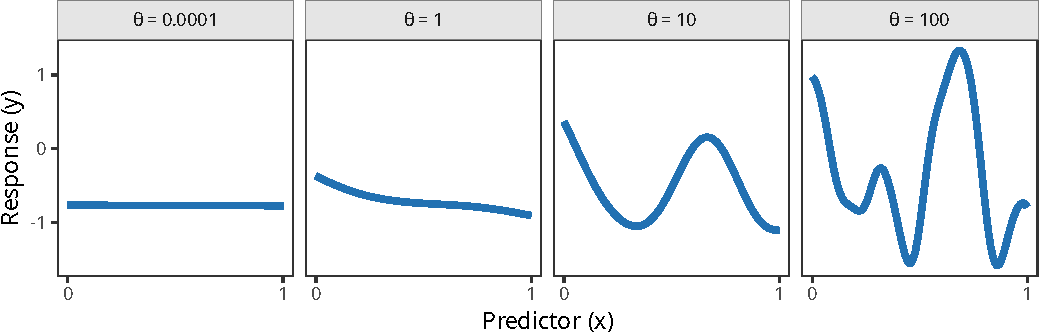
\includegraphics[height=10em]{inc/ard_response_profiles.pdf}
  \end{figure}

  \blankfootnote{Fair warning: it's not so simple! relevance = input scale
    $\times$ linearity $\times$ predictive power~\cite{piironen2016}}
\end{frame}

\begin{frame}[c]
  \frametitle{ARD + Functional inputs}
  \framesubtitle{What is the state of the art?}

  %% A tikzdiagram goes here
  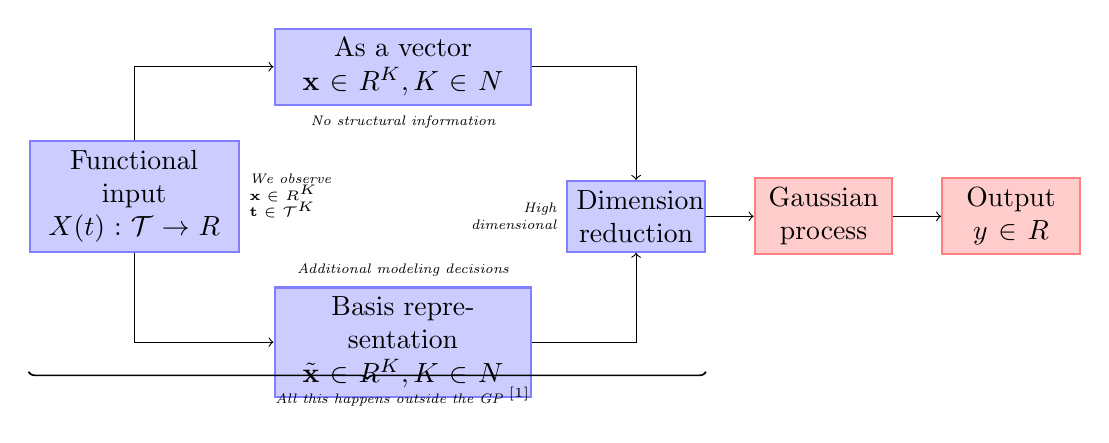
\begin{tikzpicture}
  [
  txtbox1/.style={rectangle,align=center,draw=blue!50,fill=blue!20,thick},
  txtbox2/.style={rectangle,align=center,draw=red!50,fill=red!20,thick},
  every label/.style={font=\itshape\tiny}
  ]

  \node (inp)  [txtbox1] at ( 0,  0) [text width=16ex]
  [label={[align=left]right:We observe \\ $\mathbf{x} \in \mathbb{R}^K$\\ $\mathbf{t}\in\mathcal{T}^K$}] {
    Functional input \\
    $X(t): \mathcal{T} \to \mathbb{R}$
  };
  \node (vec1) [txtbox1] [above right=4ex of inp]   [text width=20ex]
  [label=below:No structural information]{
    As a vector \\
    $\mathbf{x} \in \mathbb{R}^K, K \in \mathbb{N}$
  };
  \node (vec2) [txtbox1] [below right=4ex of inp]   [text width=20ex]
  [label=above:Additional modeling decisions]{
    Basis representation \\
    $\tilde{\mathbf{x}} \in \mathbb{R}^K, K \in \mathbb{N}$
  };

  \node (dred) [txtbox1] [above right=4ex of vec2] [text width=10ex]
  [label={[align=right]left:High\\dimensional}]
  {
    Dimension \\ reduction
  };

  \node (gp)   [txtbox2] [right=4ex of dred] [text width=10ex] {
    Gaussian \\ process
  };
  \node (out)  [txtbox2] [right=4ex of gp] [text width=10ex]  {
    Output \\ $y \in \mathbb{R}$
  };

  \node [below=6ex of vec2.north, label=below:All this happens outside the GP$~^{[1]}$] {
  };

  \draw [->] (inp.north) |- (vec1.west);
  \draw [->] (inp.south) |- (vec2.west);
  \draw [->] (vec1.east) -| (dred.north);
  \draw [->] (vec2.east) -| (dred.south);
  \draw [->] (dred.east) -- (gp.west);
  \draw [->] (gp.east)   -- (out.west);
  \path (inp.south west)
  edge[decorate,decoration={brace,mirror,raise=10ex},line width=.6pt]
  (inp.south west -| dred.south east);
\end{tikzpicture}

%%% Local Variables:
%%% mode: latex
%%% TeX-master: t
%%% End:


  \blankfootnote{
    $~^{[1]}$\cite{muehlenstaedt2017,nanty2016,wang2017,tan2019,wang2019,betancourt2020,betancourt2020a,li2021} \,
    $~^{[2]}$\cite{morris2012,kuttubekova2019}
    Add a keyword (e.g., PCA, FPCA, etc)
  }
\end{frame}

% Automatic Dynamic Relevance Determination ------------------------------------
\section{Automatic \textit{Dynamic} Relevance Determination}

\begin{frame}
  \frametitle{Automatic Dynamic Relevance Determination}
  \framesubtitle{Framework}

  A bunch of slides here
\end{frame}

% Microwave Limb Sounder -------------------------------------------------------
\section{NASA's Microwave Limb Sounder \\ {\small a case study}}

\begin{frame}[c]
  \frametitle{The science}
  \framesubtitle{Radiative transfer forward model}

  \begin{columns}[c]
    \begin{column}{0.2\textwidth}
      \begin{figure}
        \centering
        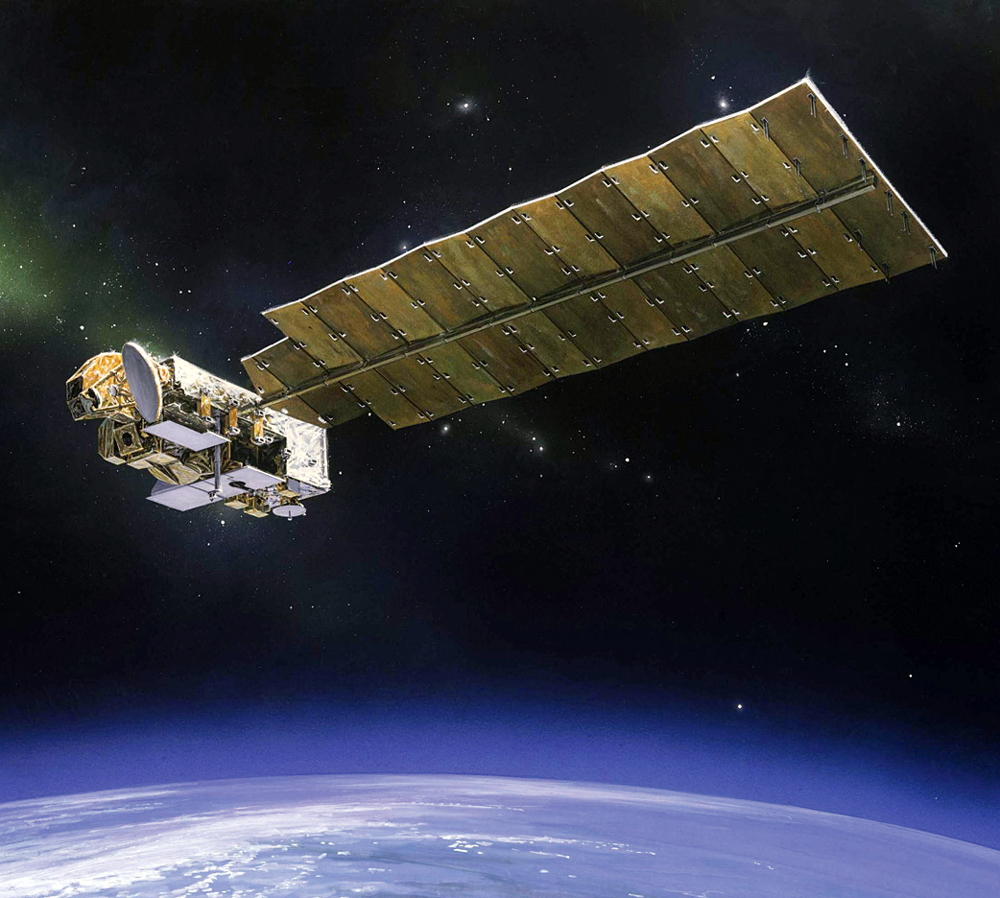
\includegraphics[height=8.5em]{inc/mls_aura}
        \caption*{
          \href{https://www.jpl.nasa.gov/missions/microwave-limb-sounder-mls}{\resizebox{!}{1.5ex}{\beamergotobutton{www}}}
          NASA JPL}
      \end{figure}
    \end{column}
    \begin{column}{0.7\textwidth}
      \begin{itemize}
      \item MLS' forward model estimates, or \emph{retrieves}, geophysical
        variables from electromagnetic radiation
      \item It calculates the radiative transfer of electromagnetic radiation
        through the atmosphere~\cite{read2006,schwartz2006}
      \item Atmospheric profiles over a vertical grid as functional inputs
      % \item Forward models are used in satellite remote sensing applications to
      %   estimate, or \emph{retrieve}, geophysical variables from satellite
      %   observations of electromagnetic radiation near 190GHz~\citep{waters2006}
      \item We consider, for some species in 190GHz~\cite{waters2006},
        pressure regions expected to be well-informed by the
        measurements~\cite{liversey2020}
      \end{itemize}
    \end{column}
  \end{columns}
\end{frame}


\begin{frame}[c]
  \frametitle{Data}
  \framesubtitle{Radiative transfer forward model}

  \begin{figure}
    \centering
    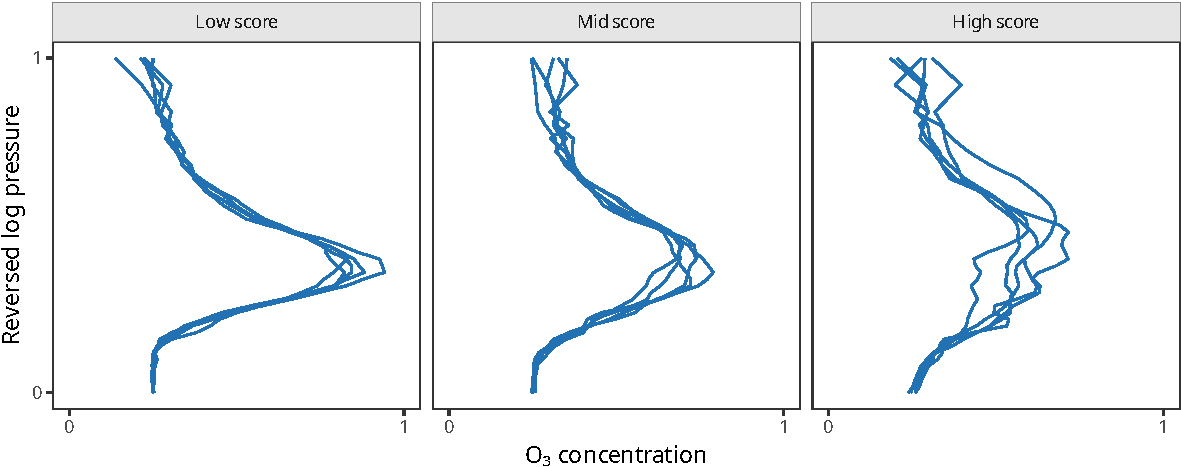
\includegraphics[height=10em]{inc/mls_input_profiles}
    % \caption*{Sample of input profiles grouped by output magnitude}
    % \begin{subfigure}{.30\textwidth}
    %   \centering
    %   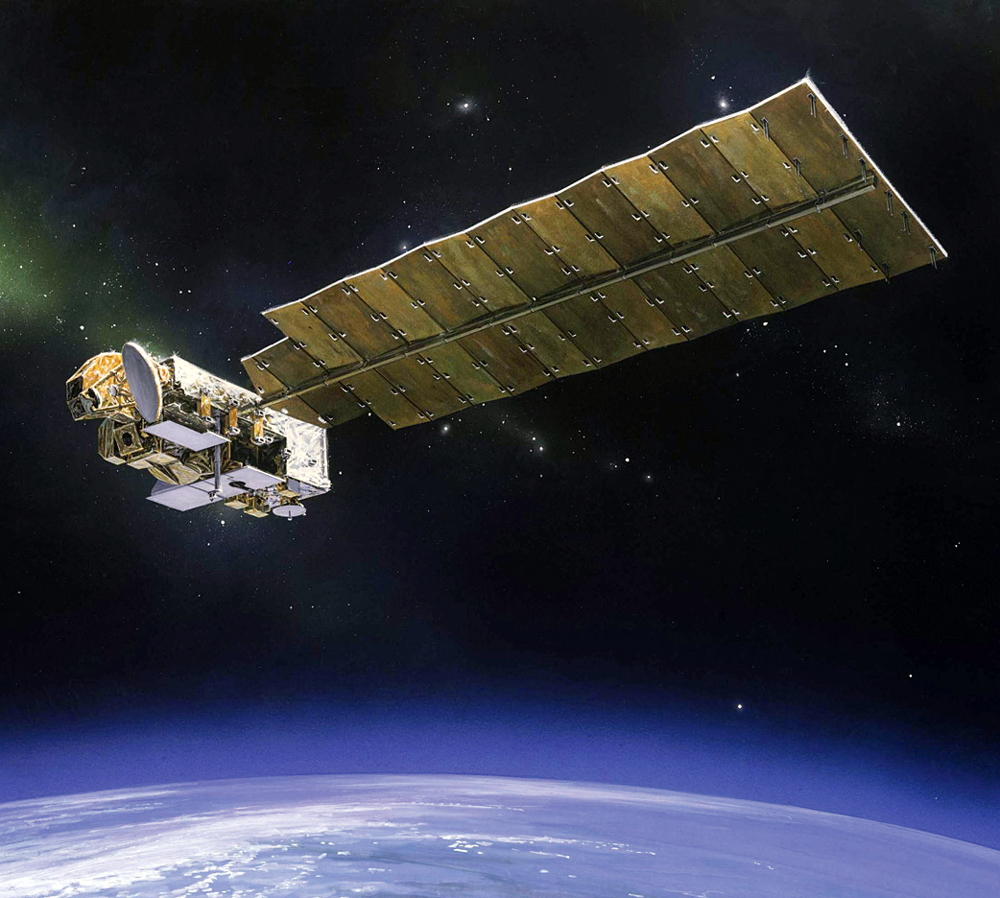
\includegraphics[height=8.5em]{inc/mls_aura}
    %   \caption*{
    %     \href{https://www.jpl.nasa.gov/missions/microwave-limb-sounder-mls}{\resizebox{!}{1.5ex}{\beamergotobutton{www}}}
    %     NASA JPL}
    %   \begin{minipage}{.1cm}
    %     \vfill
    %   \end{minipage}
    % \end{subfigure}
    % \begin{subfigure}{.65\textwidth}
    %   \centering
    %   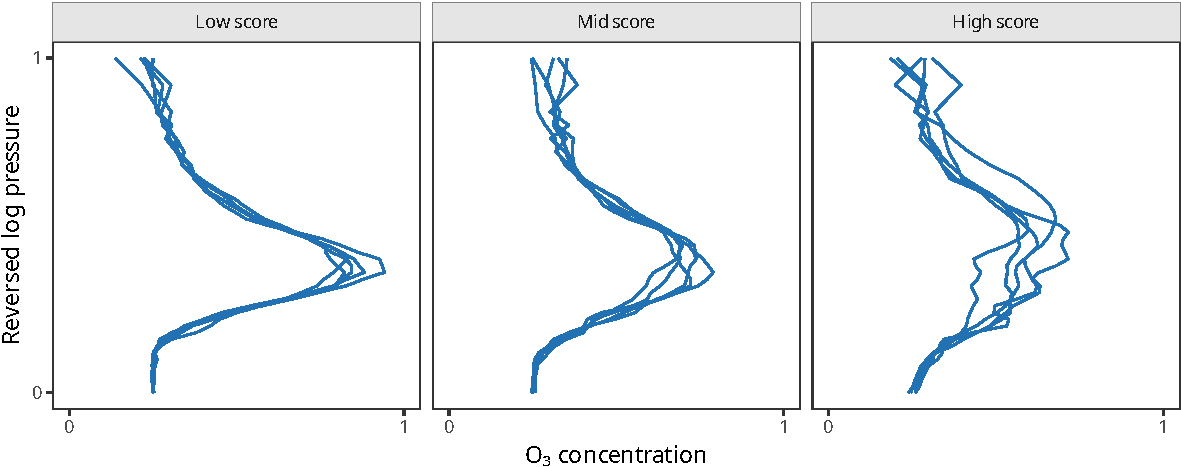
\includegraphics[height=10em]{inc/mls_input_profiles}
    %   \begin{minipage}{.1cm}
    %     \vfill
    %   \end{minipage}
    % \end{subfigure}
    % % \centering
    % % 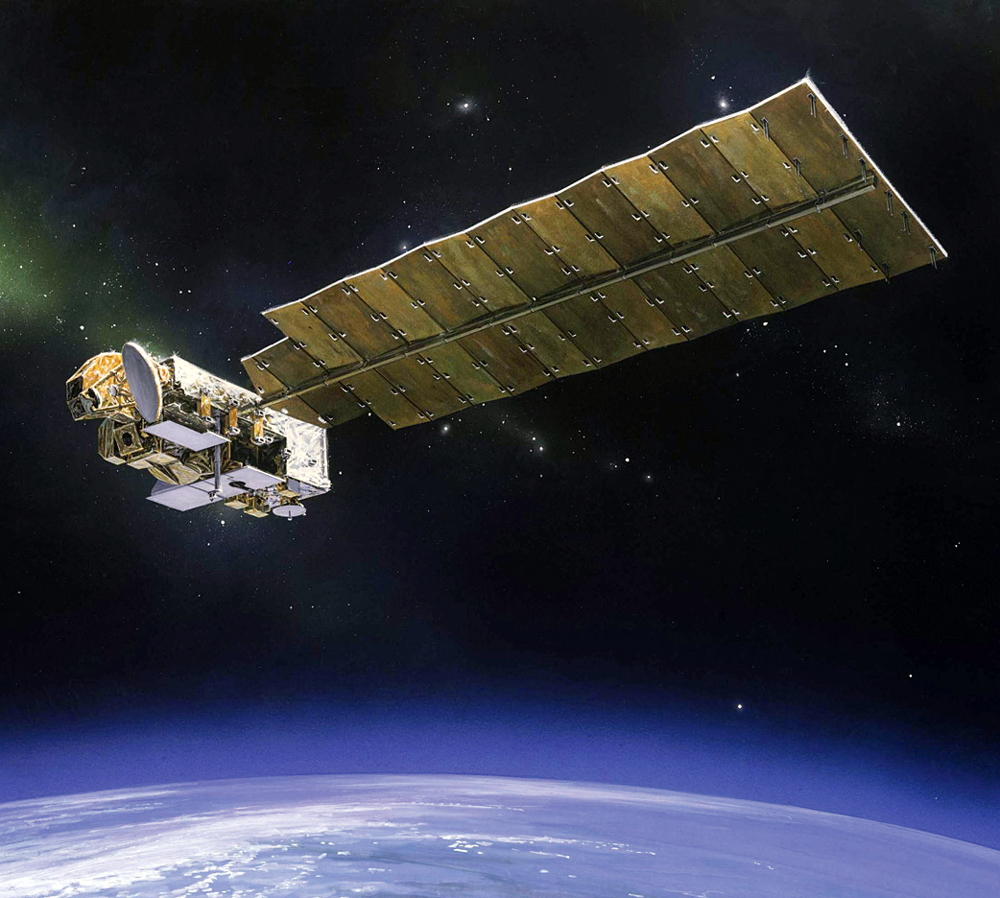
\includegraphics[height=10em]{inc/mls_aura}
    % % 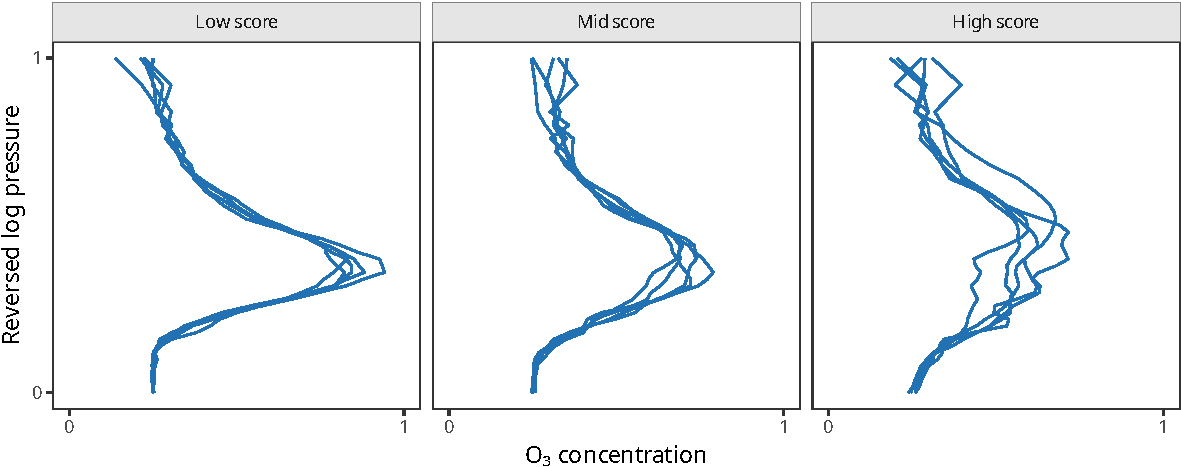
\includegraphics[height=10em]{inc/mls_input_profiles}
    % % \caption*{
    % %   \href{https://www.jpl.nasa.gov/missions/microwave-limb-sounder-mls}{\resizebox{!}{1.5ex}{\beamergotobutton{www}}}
    % %   NASA JPL}
  \end{figure}

  \begin{itemize}
  \item Radiance score variability is associated with the tropopause Ozone
    concentration
  \end{itemize}
\end{frame}

\begin{frame}[c]
  \frametitle{Methods}
  \framesubtitle{Model}

  \begin{figure}
    \centering
    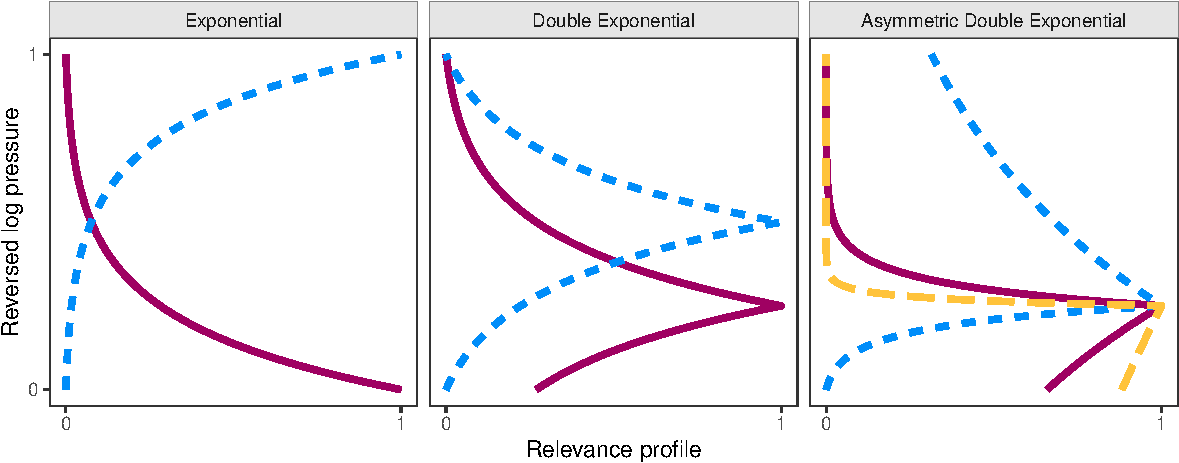
\includegraphics[height=10em]{inc/mls_weight_profiles}
  \end{figure}

  \begin{center}
    $\omega(t) = \text{exp}\left\{-(t - \tau) \lambda \kappa^s s\right\}$\\
  \end{center}

  \blankfootnote{
    Space:
    $\omega(t): \mathcal{T} = [0, 1] \to (0, 1]$,
    $s = \text{sign}(t - \tau)$,
    $\tau > 0$,
    $\lambda > 0$,
    $\kappa > 0$ \\
    \hspace{3.25ex}
    Priors:
    $\indent\tau \sim \textsc{Beta}$,
    $\lambda \sim \textsc{N}^{+}$,
    $\log(\kappa) \sim \textsc{N}$
  }
\end{frame}

\begin{frame}
  \frametitle{Methods}
  \framesubtitle{Implementation}

  \begin{itemize}
  \item 8 training and 8 test complementary sets with 1,000 soundings each
  \item 7 plausible models
    \begin{itemize}
    \item viGP SE, ARD, FPCA, FFPCA
    \item fiGP Edn, SDE, ADE
    \item One model fit separately per input-output pair
    \end{itemize}
  \item Fully Bayesian inference
    \begin{itemize}
    \item Hamiltonian Monte Carlo~\citep[ch. 5]{brooks2011}
    \item NUTS algorithm~\citep{hoffman2014} via
      Stan~\citep{standevelopmentteam2021}
    \item 1 long chain~\citep{raftery1992}
    \item Extensive search for an initial value
    \item 500 post-warmup iterations
    \item 1,500 posterior samples
    \end{itemize}
  \item Several out-of-sample validation statistics
  \end{itemize}
\end{frame}

\begin{frame}[c]
  \frametitle{Results}
  \framesubtitle{Prediction}

  \begin{table}
    \adjustbox{width=.79\textwidth,center}{%
      \centering
      \begin{tabular}{lrrrrr|r}
        \toprule
        % latex table generated in R 4.0.4 by xtable 1.8-4 package
% Sat Dec 11 14:39:57 2021
%  & H2O & HNO3 & N2O & O3 & Temp & Mean \\ 
%   \midrule
% \textsc{SE} &  .34 &  .48 &  .44 &  .32 &  .25 &  .37 \\ 
%   \textsc{ARD} &  .31 &  .47 &  .43 &  .30 &  .25 &  .35 \\ 
%   \textsc{FPCA} &  .67 &  .91 &  .99 &  .46 &  .54 &  .71 \\ 
%   \textsc{FFPCA} &  .46 &  .54 &  .46 &  .38 &  .33 &  .44 \\ 
%   \textsc{Edn} &  .33 &  .47 &  .44 &  .29 &  .25 &  .36 \\ 
%   \textsc{SDE} &  .31 &  .47 &  .44 &  .29 &  .25 &  .35 \\ 
%   \textsc{ADE} &  .31 &  .47 &  .43 &  .29 &  .25 &  .35 \\ 
%    \midrule
% Mean &  .39 &  .55 &  .52 &  .33 &  .31 &  .42 \\ 
%    \bottomrule
 & H$_2$O & HNO$_3$ & N$_2$O & O$_3$ & Temp & Mean \\ 
  \midrule
  \textsc{SE}    &  .34       &  {\bf .48} &  {\bf .44} &  .32       &  {\bf .25} &  .37 \\ 
  \textsc{ARD}   &  {\bf .31} &  {\bf .47} &  {\bf .43} &  {\bf .30} &  {\bf .25} &  .35 \\ 
  \textsc{FPCA}  &  .67       &  .91       &  .99       &  .46       &  .54       &  .71 \\ 
  \textsc{FFPCA} &  .46       &  .54       &  {\bf .46} &  .38       &  .33       &  .44 \\ 
  \textsc{Edn}   &  .33       &  {\bf .47} &  {\bf .44} &  {\bf .29} &  {\bf .25} &  .36 \\ 
  \textsc{SDE}   &  {\bf .31} &  {\bf .47} &  {\bf .44} &  {\bf .29} &  {\bf .25} &  .35 \\ 
  \textsc{ADE}   &  {\bf .31} &  {\bf .47} &  {\bf .43} &  {\bf .29} &  {\bf .25} &  .35 \\ 
   \midrule
   Mean          &  .39 &  .55 &  .52 &  .33 &  .31 &  .42 \\ 
   \bottomrule
      \end{tabular}
      \begin{tabular}{lrrrrr|r}
        \toprule
        % latex table generated in R 4.0.4 by xtable 1.8-4 package
% Sat Dec 11 14:39:57 2021
  %                & H2O & HNO3 & N2O & O3 & Temp & Mean \\ 
  % \midrule
  % \textsc{SE}    & 273 & 613 & 589 & 142 & -4 & 323 \\ 
  % \textsc{ARD}   & 196 & 619 & 581 & 92 & -14 & 295 \\ 
  % \textsc{FPCA}  & 1024 & 1320 & 1406 & 637 & 802 & 1038 \\ 
  % \textsc{FFPCA} & 535 & 646 & 630 & 295 & 268 & 475 \\ 
  % \textsc{Edn}   & 260 & 623 & 585 & 90 & 4 & 312 \\ 
  % \textsc{SDE}   & 202 & 623 & 585 & 85 & 4 & 300 \\ 
  % \textsc{ADE}   & 202 & 610 & 581 & 89 & 2 & 297 \\ 
  %  \midrule
  %  Mean & 385 & 722 & 708 & 204 & 152 & 434 \\ 
  %  \bottomrule
                 & H$_2$O & HNO$_3$ & N$_2$O & O$_3$ & Temp & Mean \\ 
  \midrule
  \textsc{SE}    & 273       & {\bf 614} & {\bf 585} & 138      & {\bf -7}  & 323 \\ 
  \textsc{ARD}   & {\bf 196} & {\bf 619} & {\bf 581} & {\bf 92} & {\bf -13} & 295 \\ 
  \textsc{FPCA}  & 1024      & 1320      & 1406      & 637      & 802       & 1038 \\ 
  \textsc{FFPCA} & 535       & {\bf 646} & {\bf 630} & 295      & 268       & 475 \\ 
  \textsc{Edn}   & 261       & {\bf 623} & {\bf 585} & {\bf 90} & {\bf 4}   & 312 \\ 
  \textsc{SDE}   & {\bf 202} & {\bf 623} & {\bf 585} & {\bf 85} & {\bf 4}   & 300 \\ 
  \textsc{ADE}   & {\bf 202} & {\bf 610} & {\bf 581} & {\bf 87} & {\bf 2}   & 297 \\ 
   \midrule
   Mean & 385 & 722 & 708 & 204 & 152 & 434 \\ 
   \bottomrule
      \end{tabular}}
    \caption*{%
      Mean validation statistics:~RMSE (left) and negative PPLD (right).\\
      Smaller values are better. Bold is best in class.
    }%
    \label{tab:validation-statistics-mini}
  \end{table}

  \blankfootnote{
    $
    \hat{v}_1
    = {\tilde{M}}^{-1} \sum_{{\tilde{m}}=1}^{{\tilde{M}}} N^{-\frac{1}{2}}
    \norm{%
      \EV{\bm{y}_{*} | \bm{X}, \bm{X}_{*}, \bm{y}, {\bm{\theta}}_{{\tilde{m}}}}
      - \bm{y}_{*}}
    $ \\
    \hspace{3.25ex}
    $
    \hat{v}_2 = {\tilde{M}}^{-1} \sum_{{\tilde{m}}=1}^{{\tilde{M}}}
    p(\bm{y}_{*} | \bm{X}, \bm{X}_{*}, \bm{y},
    {\bm{\theta}}_{{\tilde{m}}})
    $
 }

\end{frame}

\begin{frame}
  \frametitle{Results}
  \framesubtitle{Posterior for model interpretation}

  Figure with posterior weights for fiGP

  If you only did optimization, you'd only get the pluses. By running full
  bayes, I get the uncertainty (interval)

  Consider showing the as a continuous function

  Consider one posterior sample
\end{frame}

\begin{frame}
  \frametitle{Results}
  \framesubtitle{Posterior for model comparison}

  Figure with posterior weights for fiGP vs viGP
\end{frame}

% Daily Erosion Project --------------------------------------------------------
\section{Daily Erosion Project \\ {\small a case study}}

\begin{frame}
  \frametitle{The science}
  \framesubtitle{Iowa losses the thickness of a dime in soil per year (1-billion
    dollar, .5\% GDP)}

  %% Detachment
  %% https://www.dailyerosion.org/map/#20211201/20221130/avg_loss/-93.10/42.09/7.766666666666668//0/
  %% Soil loss https://www.dailyerosion.org/map/#20211216/20221215/avg_delivery/-93.56/42.05/7.766666666666668//0/
  %% https://www.desmoinesregister.com/story/money/agriculture/2014/05/03/erosion-estimated-cost-iowa-billion-yield/8682651/
  %% July 4th
  \begin{figure}
    \centering
    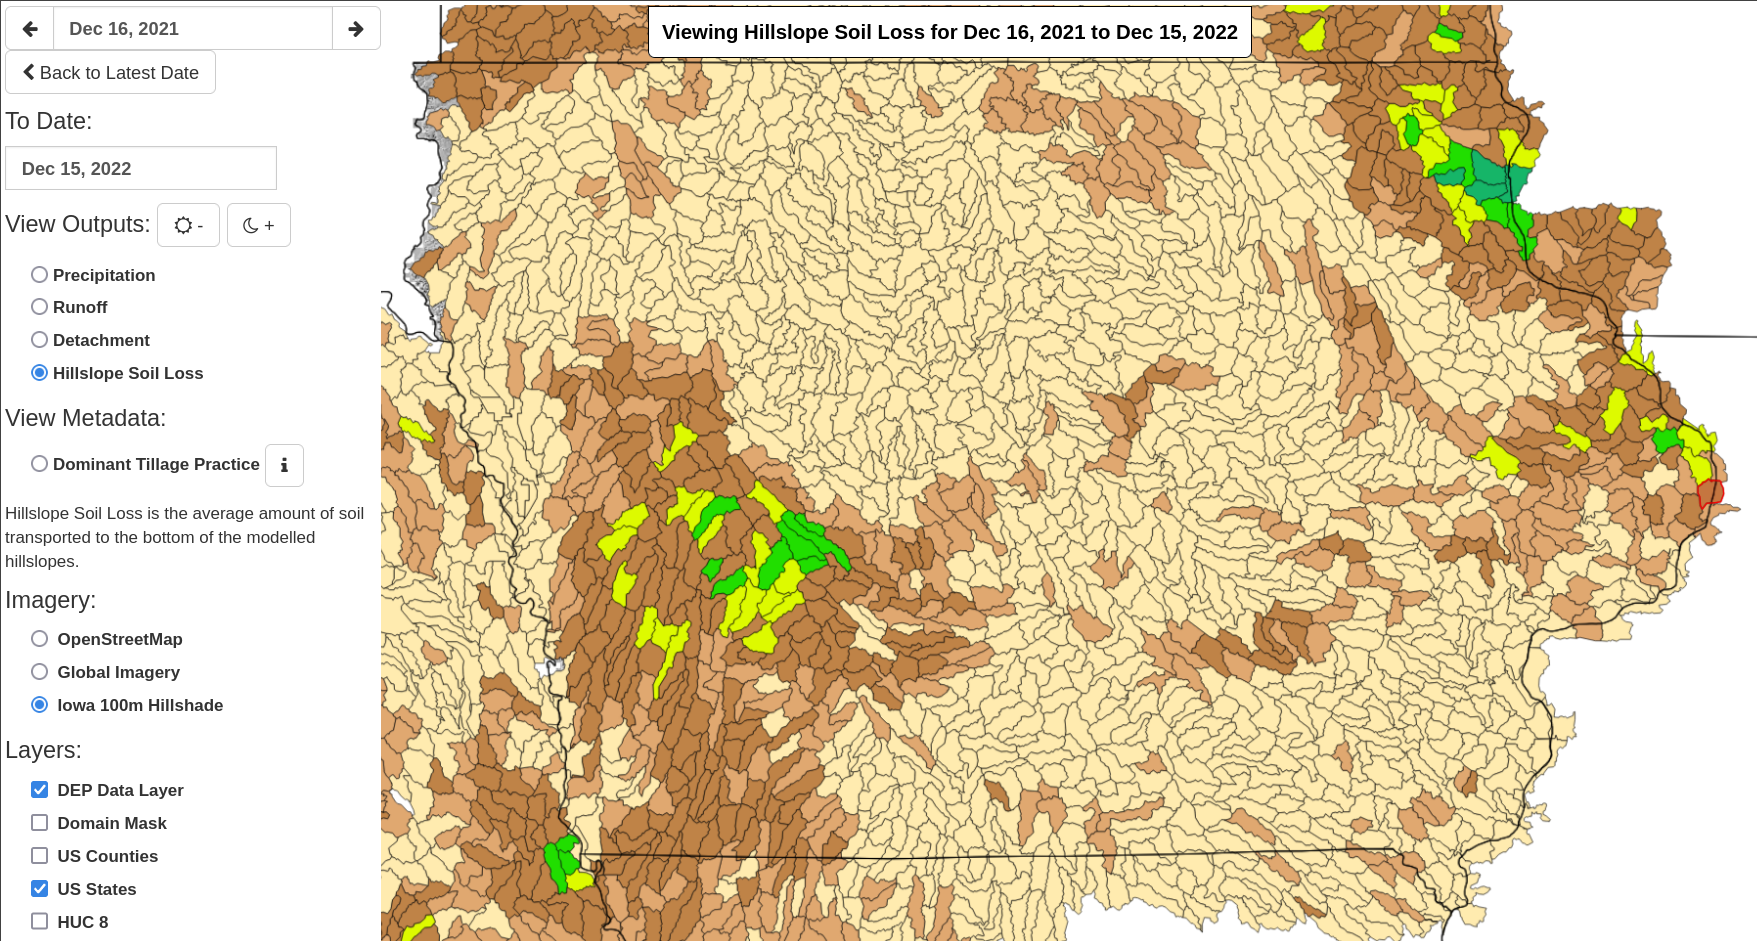
\includegraphics[height=17em]{inc/dep_soilloss_map_20221215_168.png}
      \caption*{%
        \href{https://bit.ly/3HZyaRl}{\resizebox{!}{1.5ex}{\beamergotobutton{www}}}
        Interactive map from dailyerosion.org (change to hillslope soil loss)}
  \end{figure}
\end{frame}

\begin{frame}
  \frametitle{Data}
  \framesubtitle{How does landscape affect soil loss?}

  \begin{figure}
    \centering
    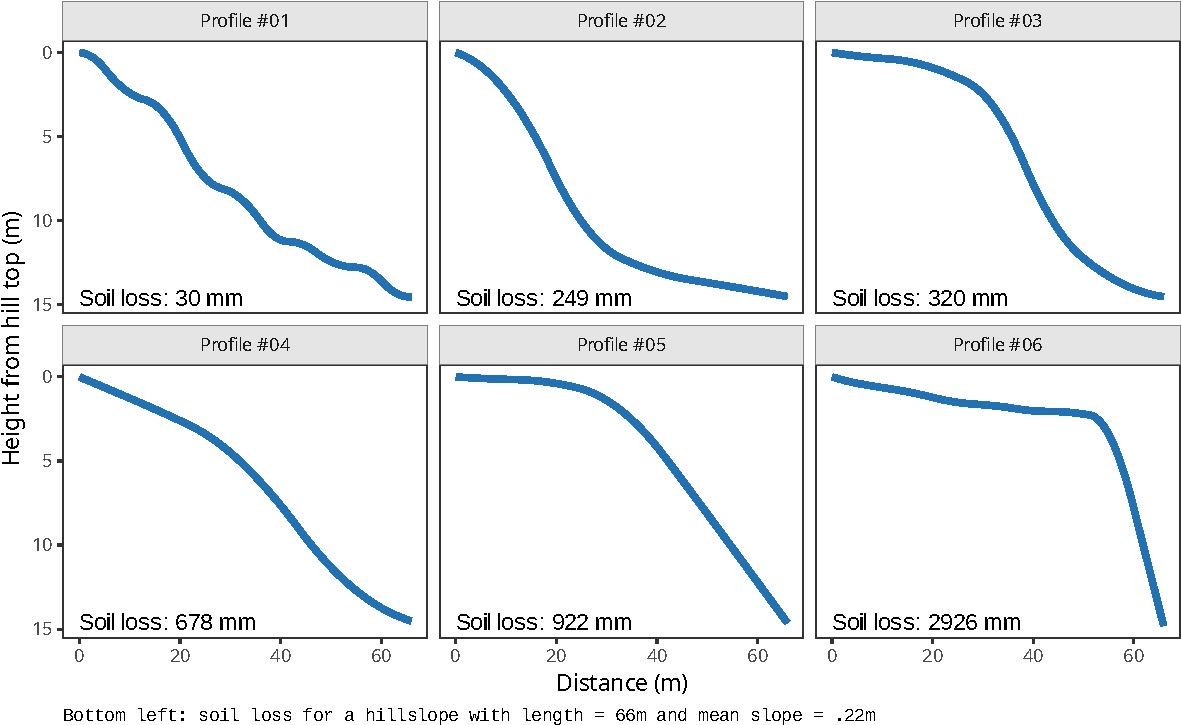
\includegraphics[height=16em]{inc/wepp_elevation_profiles}
  \end{figure}

  {\tiny
    Model documentation}
\end{frame}

\begin{frame}
  \frametitle{Methods}
  \framesubtitle{Model}

  Multiple vector (scalar), functional inputs

  Exact integral for piecewise linear models

  Math goes here

  Possibly, FEW profiles
\end{frame}

\begin{frame}
  \frametitle{Methods}
  \framesubtitle{Implementation}

  Implementation (but skip it!)
\end{frame}

\begin{frame}
  \frametitle{Results}
  \framesubtitle{Posterior for model interpretation}

  Figure with posterior weights for fiGP, and also weights for vector inputs
\end{frame}

\begin{frame}
  \frametitle{Results}
  \framesubtitle{Prediction}

  Validation table
\end{frame}

% Discussion -------------------------------------------------------------------
\begin{frame}
  \frametitle{Discussion}
  \framesubtitle{My work}

  Toward a framework for Gaussian processes with functional inputs
  \begin{itemize}
  \item Framework for Gaussian processes with functional inputs
  \item Multiple scalar, vector, and functional inputs
  \item Exact integral for piecewise linear inputs
  \item Flexible functional weight forms: ALF, ASE, FEW
  \item Case studies: Microwave Limb Sounder, Water Erosion Prediction Project
  \end{itemize}
  \vspace{3ex}
  Future work
  \begin{itemize}
  \item Functional of multiple indexes (CYCLES model 4D geometry, Grass2Gas
    grant)
  \item Multiple modes in relevance profile (MLS Temperature, mixture)
  \item Couple with local approximation (non-stationary, large matrices)
  \item DoE:~A design to learn $\omega(t)$? Use $\omega(t)$ to inform the
design?
  \item Functional input with functional output?
  \item How to bring ADRD to (D)NNs?
  \end{itemize}
\end{frame}

% Closing slides ---------------------------------------------------------------
\begin{frame}[c]
  \frametitle{Acknowledgments}
  \centering

  {\small
    Benjamin Neo, Jarad Niemi, Max D. Morris (ISU) \\
    Margaret Johnson, Joaquim Texeira, Microwave Limb Sounder team
    (JPL, Caltech) \\
    Rick Cruise, Brian Gelder, Daryl Hermann (ISU) \\
    C-CHANGE:~Science for a Changing Agriculture \\
    Foundation for Food and Agriculture Research
  }

  \vfill

  {\huge Thank you!}

  \vfill

  {\tiny References and extra slides on the back}

  \href{ldamiano@iastate.edu}{\beamergotobutton{mail}
    ldamiano@iastate.edu}

  \href{https://github.com/luisdamiano/ANL22}{\beamergotobutton{repo}
https://github.com/luisdamiano/ANL22}
\end{frame}

\setbeamertemplate{bibliography item}{\insertbiblabel}
\begin{frame}[allowframebreaks]{References}
  \tiny
  \bibliographystyle{unsrt}
  \bibliography{references}
\end{frame}

% Appendix ---------------------------------------------------------------------
\section{Appendix}
\begin{frame}
  \frametitle{Trapezoidal approximation}

  \begin{figure}[h!]
    \centering
    \caption[]{Trapezoidal approximation}
  \end{figure}

  {
    \setlength{\abovedisplayskip}{-1cm}
    \begin{align}
      \int_{\mathcal{T}}
      \omega(t)
      {\left(X_i(t) - X_j(t) \right)}^2 dt
      \approx
      &
      \sum_{k = 2}^{K} {
      \left(t_{k} - t_{k - 1}\right)
      \frac{
      \Delta_{i, j, k} +
      \Delta_{i, j, k - 1}
      }{2}
      } \\
      \Delta_{i, j, k} =
      & \
      \omega(t_{k-1}) {\left(x_{i, k} - x_{j, k}\right)}^2
    \end{align}
  }

  \blankfootnote{See~\cite{muehlenstaedt2017} for a B-spline
    approach}
\end{frame}

\end{document}
